\documentclass[12pt,a4paper]{article}

% Essential packages
\usepackage[utf8]{inputenc}
\usepackage[T1]{fontenc}
\usepackage{graphicx}
\usepackage{amsmath}
\usepackage{amsfonts}
\usepackage{amssymb}
\usepackage{hyperref}
\usepackage[margin=2cm]{geometry}
\usepackage{array} % Required for better column control
\usepackage{geometry} % To control page margins if needed
\usepackage{xcolor} % For text coloring
\usepackage{natbib} % For bibliography management

% Document information
\title{Synthetic Biology Lab Report}
\author{Harsh Agrawal (CID\: 02320622)}
\date{\today}

\begin{document}
\sloppy

\maketitle

\section{CRISPR Gene Editing of BFP to GFP in the Yeast Genome}
\subsection{Our Guide and Donor DNA Designs}

\begin{table}[h]
    \centering
    \begin{tabular}{|p{3cm}|p{11cm}|}
        \hline
        \textbf{Name}    & \textbf{\centering{Sequence}}                                                                                                        \\
        \hline
        gRNA for BFP FWD & \texttt{TTTGGTCTCACGCA\textcolor{blue}{CATGAGATAAAGTTGTTACT}GTTTTAGAGCTAGAAA
        TAGCAAGTTA}                                                                                                                                             \\
        \hline
        BFP-GFP swap FWD & \texttt{TACGGGTAAATTACCTGTTCCTTGGCCAACCCTAGTAACAACGTT\textcolor{green}{GA}\textcolor{blue}{CT}\textcolor{green}{T}
        \textcolor{blue}{AT}GGTGTTCA}                                                                                                                           \\
        \hline
        BFP-GFP swap REV & \texttt{TTTTCATATGGTCTGGGTATCTTGAGAAACATTGAACACC\textcolor{blue}{AT}\textcolor{green}{A}\textcolor{blue}{AG}\textcolor{green}{TC}AAC
        GTTGTTACTA}                                                                                                                                             \\
        \hline
    \end{tabular}
    \caption{Designed gRNA sequences along with BFP-GFP donor DNA forward and reverse primers by me (Harsh) and my lab partner (Felix). In the gRNA, the textcolor \textcolor{blue}{blue} indicates the variable detection sequence. In the donor DNAs, the textcolor \textcolor{blue}{blue} indicates the original codons for BFP (S and H) whereas \textcolor{green}{green} indicates the BFP $\rightarrow$ GFP edit.}\label{tab:gene_sequences_1}
\end{table}

\subsection{Comments on our CRISPR Construct Design}
\subsubsection{Differences in the design}
\begin{itemize}
    \item We assumed that we couldn't use the PAM site immediately next to the edit site
          and thus used a PAM site (5'--AGG--3') on the complementary strand 13 bases
          downstream of the edit site. Our assumption was wrong and in retrospect, we
          should have chosen the PAM site we identified originally that was chose to the
          edit site.
    \item Our donor DNA forward primer was almost identical to the one provided in the
          lab but using different two different Threonine codons ACT instead of ACA (for
          the Serine to Threonine switch) and ACG rather than ACT (for another Theronine
          3 bases upstream of the edit site). More over, our forward primer began two
          bases later than the one provided in the lab and thus spanned an extra two
          bases at the end.
\end{itemize}
\subsubsection{Differences in Outcome if we used our gRNA and donor DNA sequences}
\begin{itemize}
    \item Due to our PAM site being further away from the edit site (as compared to the
          one provided in the lab), Cas9 cleavage efficiency would decrease, potentially
          lowering the number of fluorescent colonies or preventing editing entirely.
    \item While there is difference in relative abundances of the different codons in
          both designs, I believe the difference in outcome might not be as significant
          as efficiency decrease due to wrong choice of PAM site placement would dominate
          the edit.
\end{itemize}
\subsection{Annotated Photo of the Agar Plates}
\begin{figure}[h]
    \centering
    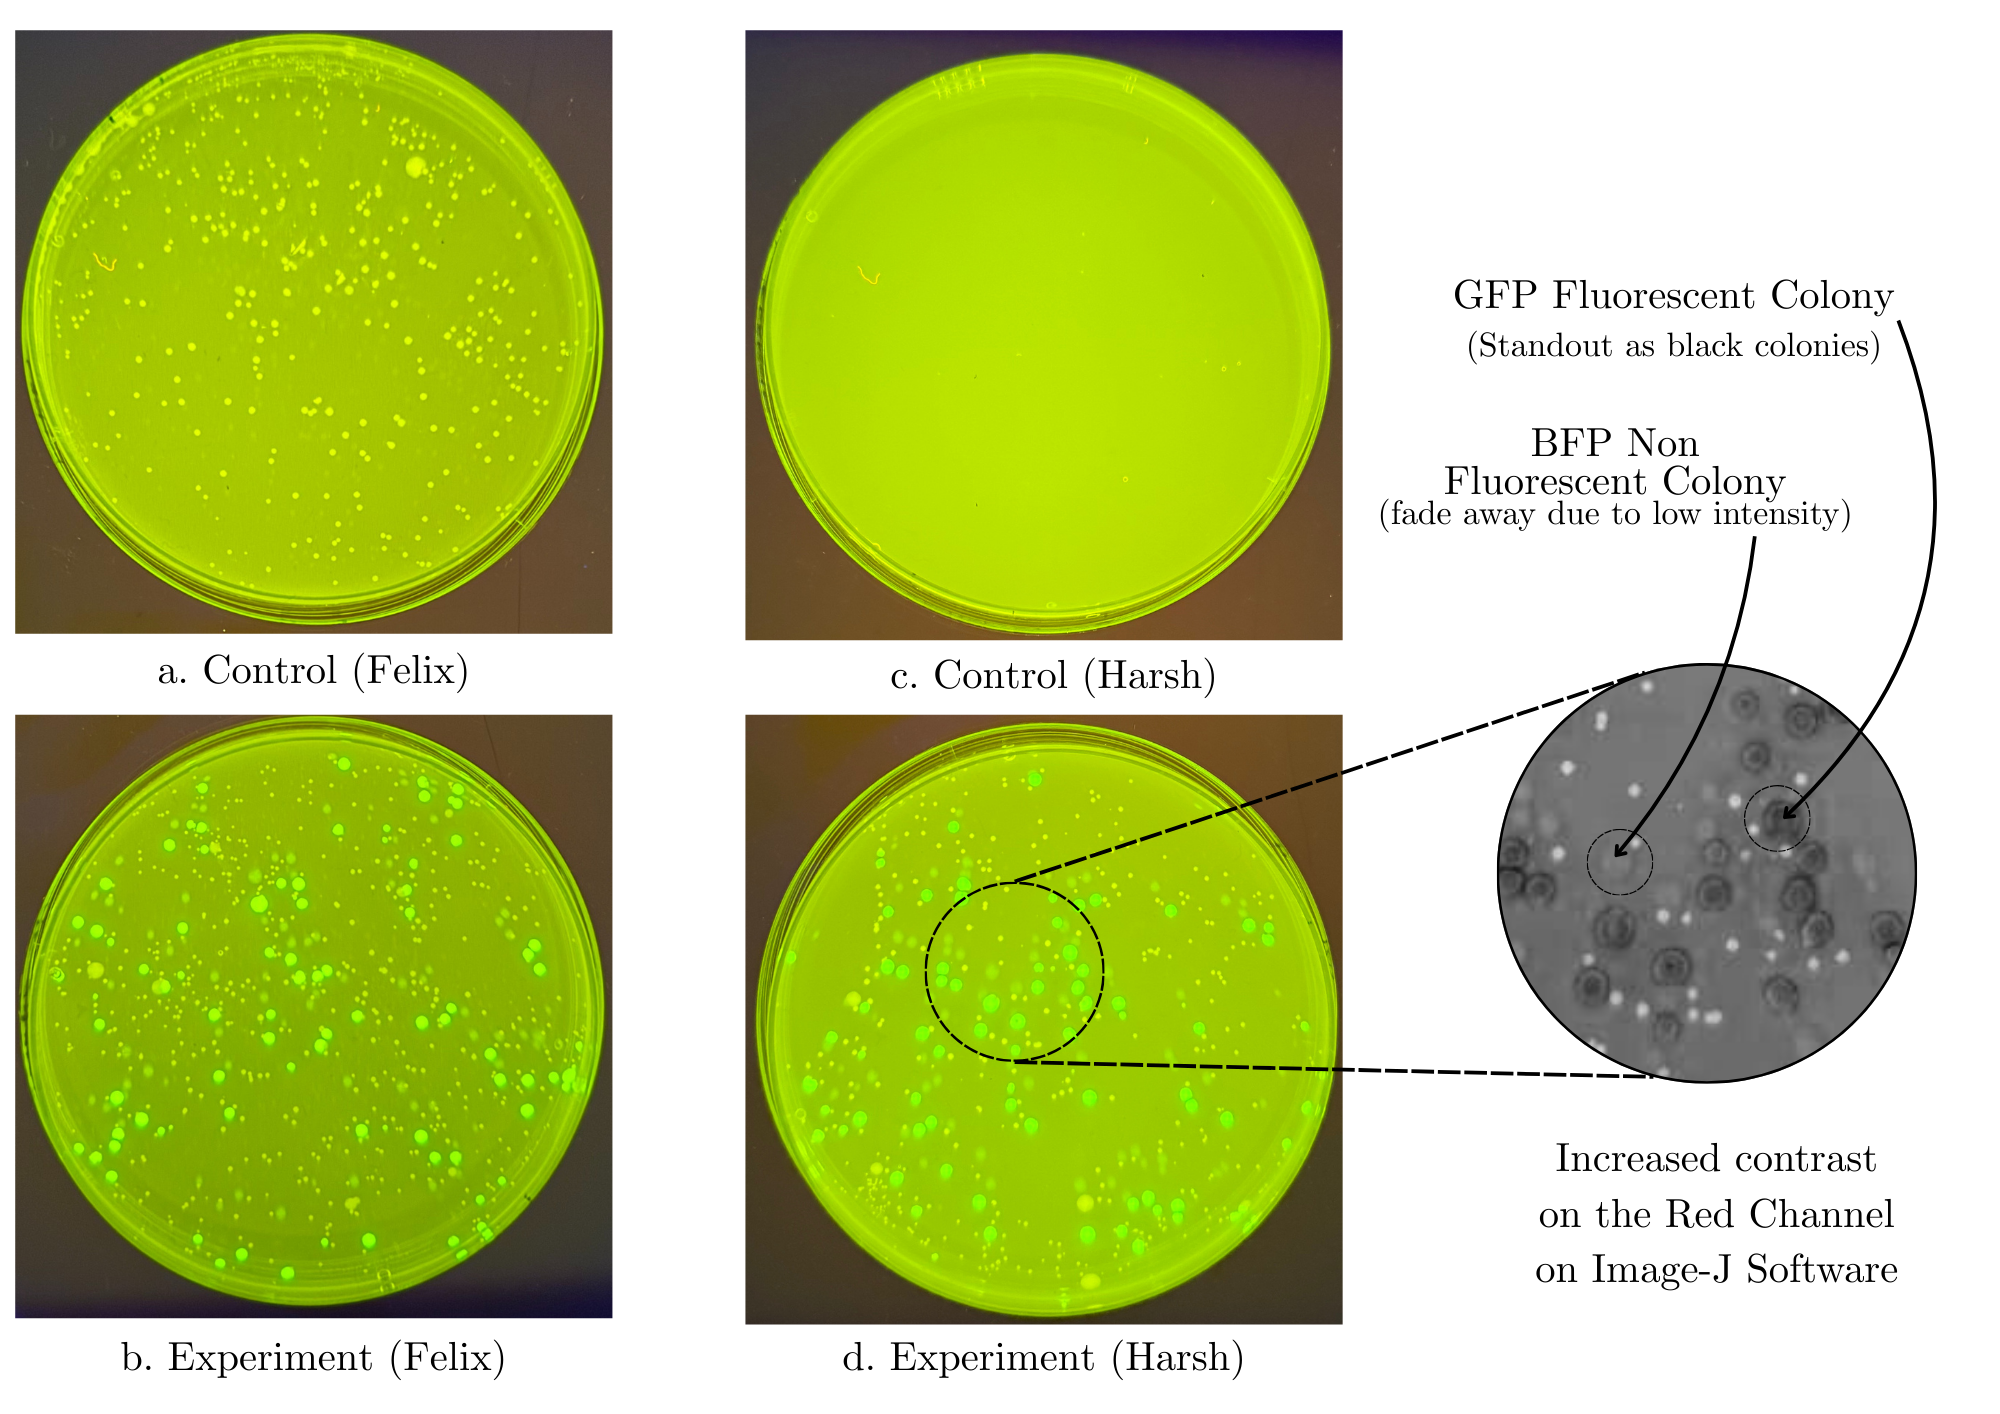
\includegraphics[width=0.8\textwidth]{figures/exp_1_agar_plates.png}
    \caption{Annotated photos of the Agar Plates for me (Harsh) and my partner (Felix). The image was converted to the red-channel in ImageJ with high contrast to highlight the green fluorescent colonies from non-fluorescent colonies as labeled in the image above.}\label{fig:exp_1_agar_plates}
\end{figure}

\subsection{Table of the Results}
\begin{table}[h]
    \centering
    \begin{tabular}{|l|c|c|c|c|}
        \hline
        \textbf{Colony Type} & \textbf{Felix C} & \textbf{Felix X} & \textbf{Harsh C} & \textbf{Harsh X} \\
        \hline
        Non-Fluorescent      & 51               & 23               & 0                & 71               \\
        \hline
        Fluorescent          & 0                & 69               & 0                & 71               \\
        \hline
        \textbf{Total}       & \textbf{51}      & \textbf{92}      & \textbf{0}       & \textbf{142}     \\
        \hline
    \end{tabular}
    \caption{\centering Counts for fluorescent and non-fluorescent colonies on each plate with assistance from IMAGEJ software.}\label{tab:colony_counts}
\end{table}
\subsection{Discussion of the Results}
\textit{*Note: I have Deuteranopia (red-green colorblindness), due to which I couldn't visually identifying any fluorescent colonies. For the same reason, I chose to convert the image to the red-channel in ImageJ with high contrast to highlight the green fluorescent colonies from non-fluorescent colonies (it seems counterintuitive as I should have used a green channel but the red channel had better contrast). The colonies mentioned on the table are tallied from my lab partner for correctness. This has also affected my ability to properly identify colors in the later experiments and thus there my errors in my judgement. }

The results from this transformation experiment, where CRISPR/Cas9 was used to
transform yeast BFP to GFP, show distinct outcomes for my plates and my lab
partner's. My Control (C) plate had 0 colonies, indicating a failure in uptake
of the CRISPR construct or poor growth competency of my control cells. Since an
identical CRISPR construct was used for both, this error should primarily be
due to procedural / pipetting error.

Felix's control (C) plate had 51 non-fluorescent colonies, indicating
successful CRISPR construct uptake and repair via non-homologous end joining by
the yeast cells due to the absence of donor DNA. This clearly shows that CRISPR
construct uptake allowed growth on uracil-deficient media, but the BFP-to-GFP
editing did not occur as expected.

My experimental (X) plate had 142 colonies (71 fluorescent, 71
non-fluorescent), indicating $\approx 50\%$ success rate in the editing of BFP
to GFP. This indicates that half of the cell colonies underwent non-homology
end joining to repair the cut DNA whereas the other half included the CRISPR
edit via homology directed repair. Felix's experimental (X) plate had 92
colonies (69 fluorescent, 23 non-fluorescent), reflecting a 75\% editing
success rate due to efficient homologous recombination. While the number of
colonies on Felix's plate is less than mine, the success rate in higher.

Moreover, the colonies on Felix's Experimental (X) plate was almost double the
amount in the Control (C) plate indicating that the control cells might have
continually underwent DNA cleavage, and died therefore, due the presence of the
CRISPR construct but not the donor DNA.

Since all the experimental setup was identical along with the reagents used,
the difference in colony and efficiency between mine and Felix's cells can most
likely be attributed to procedural differences.

\section{Golden Gate Assembly of the Defined and Combinatorial Metabolic Pathways}

\subsection{Reasoning behind the Defined (D) Design choices}
\begin{table}[h]
    \centering
    \begin{tabular}{|l|c|c|}
        \hline
        \textbf{Gene} & Harsh Strength Choice (Promoter) & Felix Strength Choice (Promoter) \\
        \hline
        Crt-E         & Strong (pHTB2)                   & Weak (pRAD27)                    \\
        \hline
        Crt-I         & Strong (pTEF2)                   & Medium (pALD6)                   \\
        \hline
        Crt-YB        & Strong (pHHF2)                   & Strong (pHHF2)                   \\
        \hline
    \end{tabular}
    \caption{\centering Genes and their promoters used (indicating strength) in the defined (D) design.}\label{tab:defined_design}
\end{table}

Here are the reasons for the choice of promoters by me (Harsh):
\begin{itemize}
    \item The primary reason was to maximize metabolic flux through the defined pathway.
          Selecting all strong promoters ensures a high initial flux of geranylgeranyl
          diphosphate (via CrtE), rapid conversion of phytoene to lycopene (via CrtI),
          and efficient cyclization to beta-carotene (via CrtYB). This would test the
          hypothesis that transcription is the rate-limiting step in beta-carotene
          accumulation. If successful, this would lead to a high accumulation of
          orange-yellow colonies.
    \item Another reason was to enquire which gene was the rate-limiting step in the
          pathway. For example, if CrtYB is overexpressed but beta-carotene levels remain
          low (e.g., red colonies indicating lycopene buildup), it could indicate
          insufficient activity of CrtI or CrtE, despite their strong promoters. This
          mirrors strategies in metabolic engineering where over-expression highlighted
          bottlenecks for optimization.
    \item The final reason was to test the metabolic stress on the yeast cells. Small or
          sparse colonies might be indicative of this.
\end{itemize}

Felix's choice of the promoters in increasing order of strength was aimed to
limit early pathway expression, preventing competition with native pathways
like ergosterol biosynthesis for precursors like FPP, reducing metabolic
burden. Compared to a direct design with all strong promoters, this
weak-medium-strong gradient tests whether escalating expression toward the end
improves balance and yield by mitigating bottlenecks, offering a more nuanced
approach to optimization.

\subsection{Reasoning behind the Combinatorial (C) Design choices}
\begin{table}[h]
    \centering
    \begin{tabular}{|l|c|c|}
        \hline
        \textbf{Gene} & Harsh Strength (Promoter)   & Felix Strength (Promoter)    \\
        \hline
        Crt-E         & Strong (pHTB2)              & Mixed (pPAB1, pHTB2, pRAD27) \\
        \hline
        Crt-I         & Mixed (pTEF2, pALD6, pHHF1) & Strong (pTEF2)               \\
        \hline
        Crt-YB        & Weak (pRET2)                & Weak (pRET2)                 \\
        \hline
    \end{tabular}
    \caption{\centering Genes and their promoters used (indicating strength) in the combinatorial (C) design.}\label{tab:comb_design}
\end{table}

My choice of a strong promoter for Crt-E (pHTB2), mixed promoters for Crt-I
(pTEF2, pALD6, pHHF1), and a weak promoter for Crt-YB (pRET2) hypothesized that
making flux dominant in the early part of the beta-carotene pathway would
optimize overall production. This involved driving robust geranylgeranyl
diphosphate (GGPP) synthesis with a strong Crt-E promoter to ensure a strong
initial flux, varying Crt-I expression to fine-tune the conversion of phytoene
to lycopene and prevent bottlenecks, and limiting Crt-YB activity with a weak
promoter to test whether reduced downstream expression could efficiently
utilize intermediates without causing accumulation (e.g., avoiding red lycopene
colonies). This approach contrasts with a direct design using uniform strong
promoters, aiming to explore if early-pathway dominance yields better
efficiency or healthier colonies by balancing metabolic load.

Felix's selection of a medium promoter for Crt-E, a strong promoter for Crt-I,
and a weak promoter for Crt-YB aimed to balance precursor availability and
intermediate conversion while minimizing downstream stress. The medium Crt-E
promoter was likely chosen to moderate GGPP production, reducing competition
with native pathways like ergosterol synthesis and alleviating metabolic
burden. A strong Crt-I promoter ensured high phytoene desaturase activity,
maximizing lycopene production to prevent bottlenecks at this intermediate
step. The weak Crt-YB promoter limited the final cyclization to beta-carotene,
matching the moderate upstream flux and avoiding overproduction stress,
potentially enhancing overall pathway efficiency.

\newpage
\subsection{Annotated Photos of the Results}
\begin{figure}[h!]
    \centering
    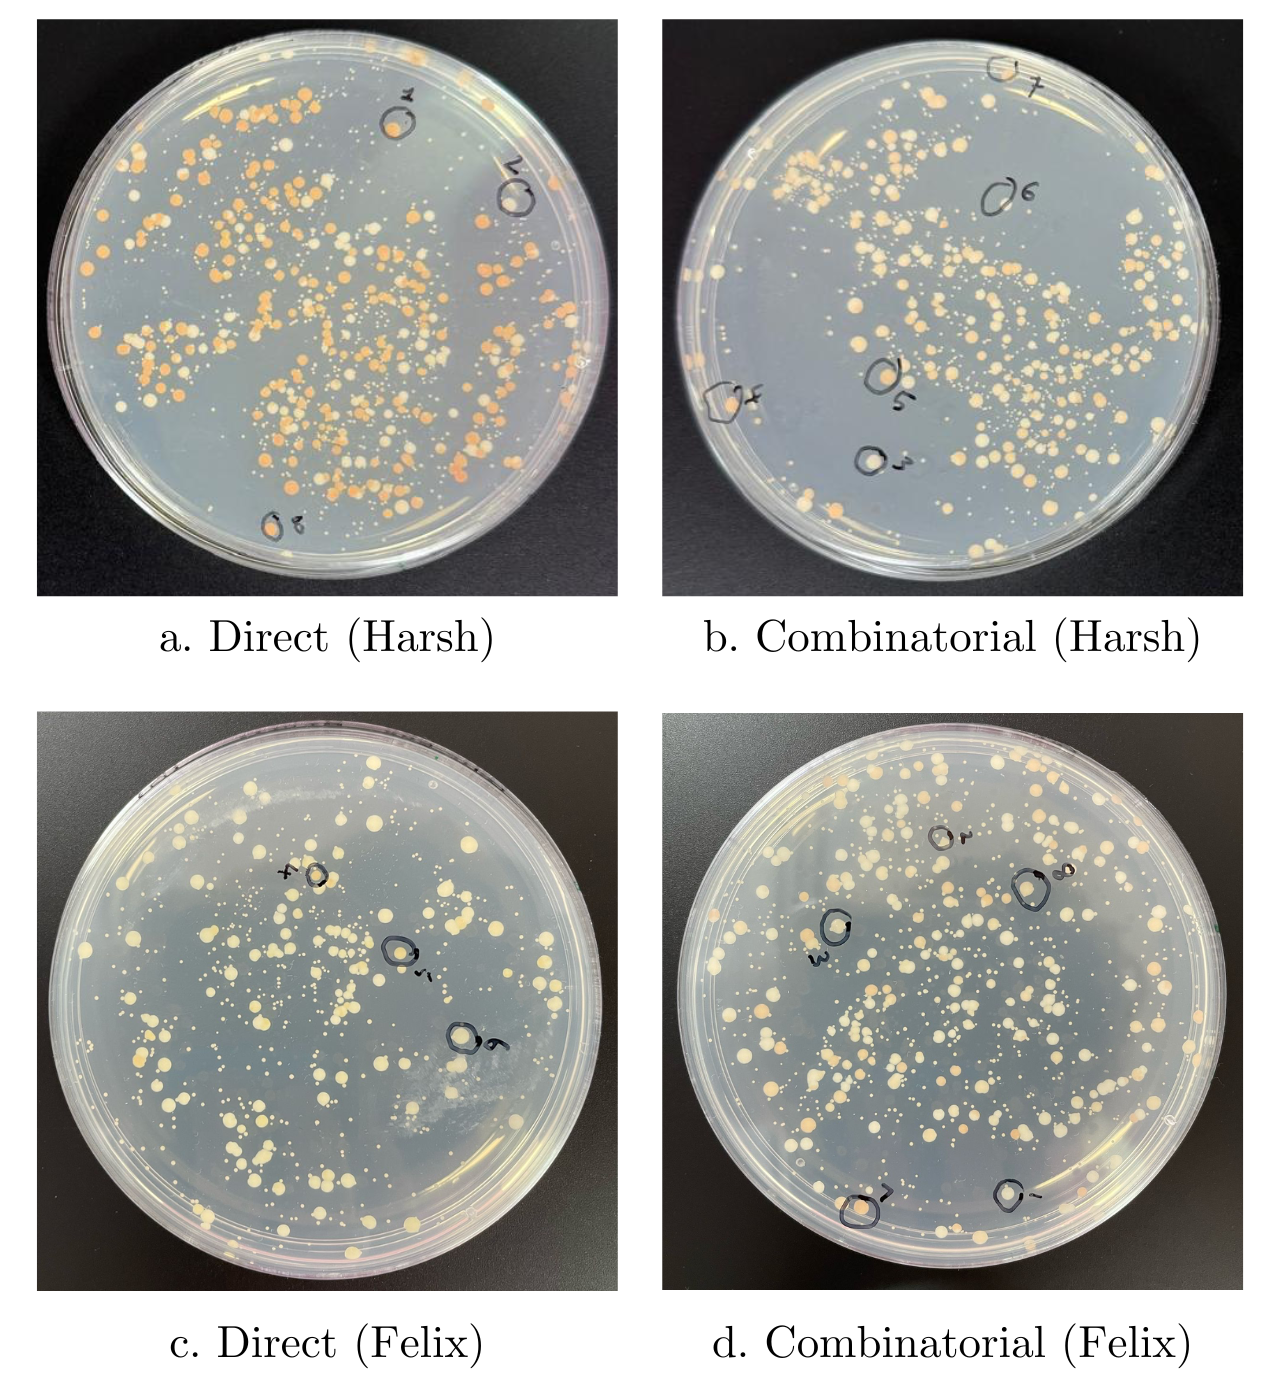
\includegraphics[width=0.8\textwidth]{figures/direct_and_combinatorial.png}
    \caption{Annotated photos showing the results of both the direct (D) and combinatorial (C) designs. The colonies chosen for streaking are marked on each plate with an associated number.}\label{fig:direct_comb_results}
\end{figure}

\subsection{Discussion of Results in Context of Assembly and Transformation}
The number of colonies on all four plates seem be quite high. This suggests
that the CRISPR transformation efficiency was quite high. This also suggests
that the PAM site must have modified as expected to prevent excessive cleavage
DNA (leading to death / low number of colonies as seen in agar plates of other
experiments). All four plates seem to show a mix range of colors from light
yellow to orange suggesting that the knockout rate was also quite high. In the
Direct (D) design, most colonies are saturated Orange apart from a few colonies
that are completely white in color. This suggests either that these colonies
underwent non-homologous end joining or that the CRISPR construct was not able
to make the edit. There also seems to be a lot of small white colonies
(contaminants) that seem to have accumulated equally on all plates.

\subsection{Choice of Colonies for Streaking}
To validate the hypothesis outline above, we carefully chose colonies for
streaking in order to maximize for color diversity from each of the colonies.
Colonies 1 and 8 (chosen from Harsh's Direct (D) design) were chosen as they
were the most orange in color and thus would be the best to validate whether
all strong promoters would lead to the highest accumulation of beta-carotene as
compared to other strategies. Colony 2 was taken as an outlier from the Direct
(D) design as it was one of the few colonies that wasn't either completely
saturated with orange or was white in color.

Colonies 3--7 were chosen from the Combinatorial (C) design to display the
different range of colors that can be seen in the Combinatorial (C) design with
mixed promoters. More colonies were chosen from the Combinatorial (C) design
from both me and Felix's plate.

\subsection{Annotated Photos of the Streaked Plates}
\begin{figure}[h]
    \centering
    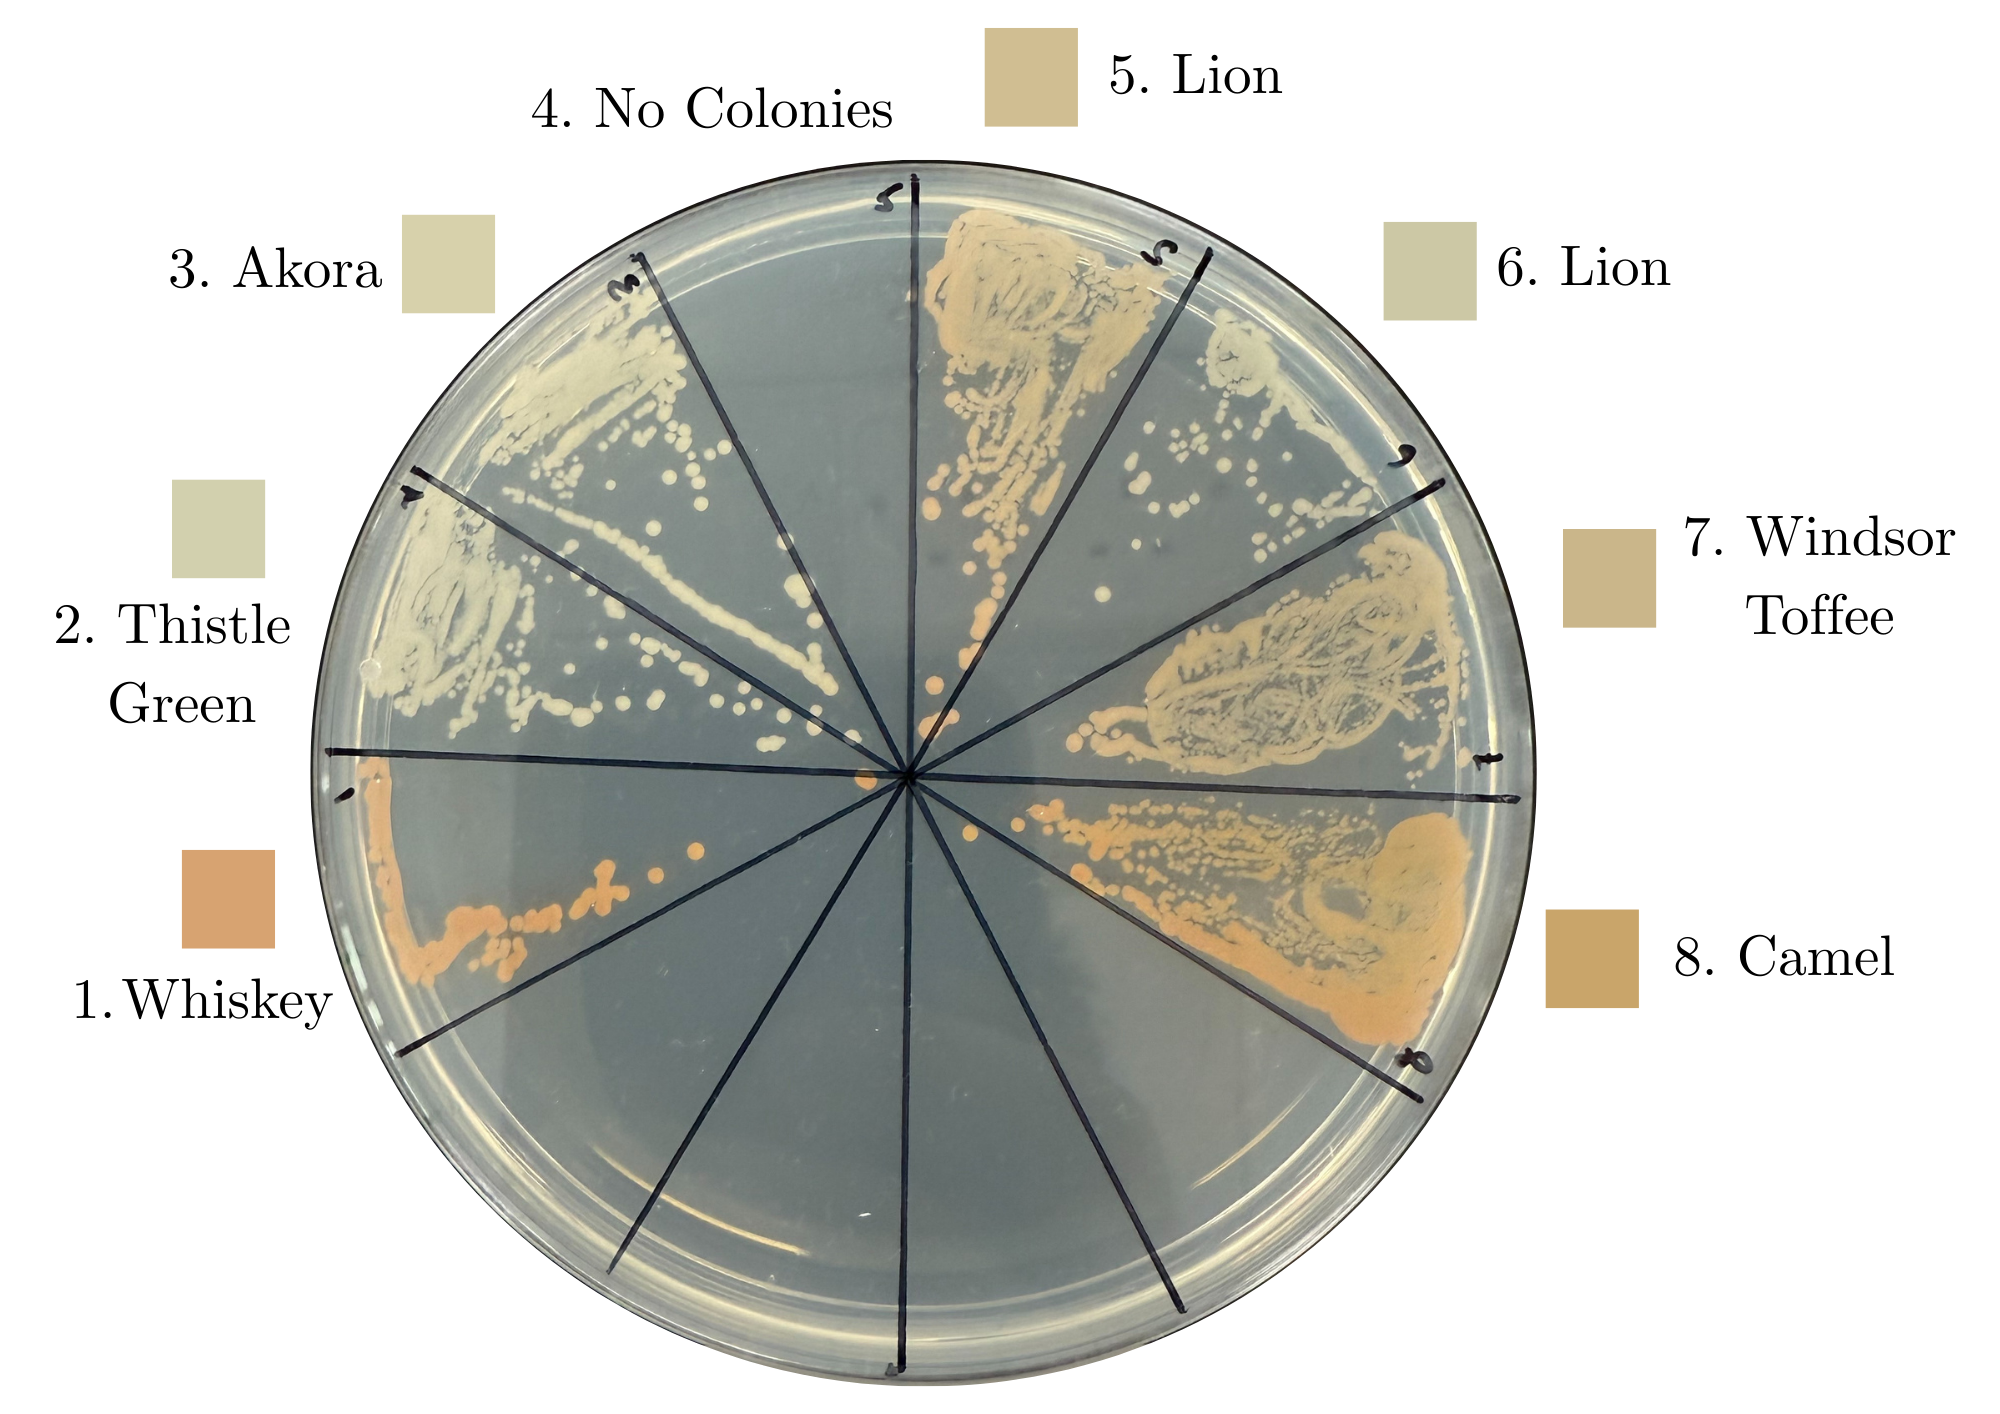
\includegraphics[width=0.9\textwidth]{/Users/harshagrawal/Downloads/code/reports/year_3/report_syn_bio/figures/streak_plates.png}
    \caption{Annotated photos showing the results of the streaked plates.}\label{fig:streaked_plates}
\end{figure}

\subsection{Discussion of the Results in Context of the Design Choices}
\textit{*Note: Felix's streaking plate was lost (unsure how) and so I'll primarily be biasing the analysis on my results.}

The results from the Direct (D) design (Plate a) strongly support Harsh's
hypothesis that transcription might be the rate-limiting step in beta-carotene
accumulation. Colonies 1 and 8, which were streaked out, suggest that
upregulating all promoters (pHTB2 for Crt-E, pTEF2 for Crt-I, pHHF2 for Crt-YB)
leads to a higher accumulation of beta-carotene compared to the other
strategies (Combinatorial - Harsh, Direct - Felix, and Combinatorial - Felix).
The colonies from the Direct (D) design were significantly more orange in color
compared to all other plates, indicating that the strong promoters drove high
expression of all three genes, resulting in efficient flux through the pathway
and minimal accumulation of intermediates like lycopene (which would appear
red). This can be visally seen in the streaked colonies 1 and 8.

In contrast, the Combinatorial (C) design (Plate b) showed more variability in
colony color, with some orange colonies but also beige and reddish ones. The
reddish colonies likely indicate lycopene accumulation, which could result from
the weak promoter for Crt-YB (pRET2) limiting the conversion of lycopene to
beta-carotene (can be seen in the colonies 2 and 3). The mixed promoters for
Crt-I (pTEF2, pALD6, pHHF1) introduced variability in phytoene desaturase
activity, which may have led to inconsistent flux through the pathway. While
this design successfully generated a range of expression profiles, it did not
achieve the same level of beta-carotene production as the Direct design,
suggesting that a balanced but lower expression profile (especially for Crt-YB)
was less effective in this context.

The Combinatorial (Felix) plate (Plate d) also shows a mix of colors, but with
less orange intensity than Harsh’s plates, reflecting Felix’s choice of a
medium promoter for Crt-E (mixed: pPAB1, pHTB2, pRAD27), a strong promoter for
Crt-I (pTEF2), and a weak promoter for Crt-YB (pRET2). This design similarly
struggled with bottlenecks, likely due to insufficient Crt-E activity and
limited Crt-YB expression.

The observation that I believe has the strongest validity is that
\textbf{having all strong promoters doesn't cause a severe metabolic stress on
    the yeast cells}. This is evidenced by the fact that all the colonies are of a
similar color and are of a similar size. This suggests that the metabolic
stress is not too high and the cells are able to handle the strong promoters.

Apart from these observations, no other significant difference was observed
between the four plates.

\section{Promoter Modification of the Carotenoid Biosynthetic Pathway}
\subsection{Our Guide RNA and Donor DNA Sequences}
We chose gRNA 18 with the RAP1 binding site on KL-TEF2p to edit. The Donor DNA
design is shown below:
\begin{table}[h]
    \centering
    \begin{tabular}{|p{3cm}|p{11cm}|}
        \hline
        \textbf{Name}  & \textbf{\centering{Sequence}}                                               \\
        \hline
        Forward Primer & \texttt{GGTTCTTTTCTCCCGCTCTCTCGCAATAACAATGAA\textcolor{red}{CACTCGTACAC}TCA
        TAGCCTACAC}                                                                                  \\
        \hline
        Reverse Primer & \texttt{CCTGTATAAACGCTACTCTGTTCACCTGTGTAGGCT\textcolor{red}{ATGAGTGTACG}AGT
        GTTCATTGTT}                                                                                  \\
        \hline
    \end{tabular}
    \caption{\centering Donor DNA sequences for the RAP1 binding site modification. The site of edit is highlighted in \textcolor{red}{red}.}\label{tab:exp_3_sequences}
\end{table}

\subsection{Choice of Promoter Modification}
RAP1, or Repressor Activator Protein 1, is an essential transcription factor in
Saccharomyces cerevisiae, known for binding to upstream activating sequences
(UAS) in promoters. Literature, such as \citet{Gonzalez2020}, highlights RAP1's
role in depleting nucleosomes from its binding sites, increasing accessibility
for other transcription factors and enhancing gene expression. This is
particularly relevant for highly expressed genes, including those involved in
metabolic pathways. For instance, \citet{Miura1998} discuss engineering yeast
for carotenoid production, emphasizing the importance of promoter strength,
which aligns with modifying RAP1 binding sites to boost transcription. Recent
work by \citet{Tang2020} has further elucidated the architecture of yeast
promoters and the role of transcription factors like RAP1 in regulating gene
expression, providing valuable insights for synthetic biology applications.

gRNA-18 was chosen because it targets a potential RAP1 binding site, offering a
direct approach to enhance transcriptional activation. The edited sequence
provided shows changes to make the target region more similar to the RAP1
consensus sequence, suggesting an intent to increase RAP1 binding affinity.
This is supported by the experimental design, where primers were designed 40
base pairs upstream and downstream of the edited region, ensuring precise
homology-directed repair (HDR) to implement the modification.

In contrast, gRNA-16 and gRNA-14 target TA-rich regions, which are likely
involved in nucleosome positioning or other regulatory mechanisms but not
directly in transcription factor-mediated activation. TA-rich regions, as
discussed in promoter architecture studies (e.g., \citet{Gonzalez2020};
\citet{Tang2020}), can affect chromatin accessibility, but their impact on
transcription factor binding, especially RAP1, is less direct. Therefore,
gRNA-18 was preferred for its specificity to a functionally critical region for
upregulating CrtYB expression.
\subsection{Concentration and Quality of Donor DNA}
\begin{table}[h]
    \centering
    \begin{tabular}{|l|c|c|}
        \hline
        \textbf{Measurement}      & \textbf{Value (Harsh)} & \textbf{Value (Felix)} \\
        \hline
        DNA Concentration (ng/ul) & 303.6                  & 402                    \\
        \hline
        Quality (A260/A280)       & 1.832                  & 1.805                  \\
        \hline
    \end{tabular}
    \caption{\centering Concentration and quality of the donor DNA for me and my lab partner.}\label{tab:dna_concentration}
\end{table}
\subsection{Calculation of Annealing Temperature}
The annealing temperature was calculated to be $51.8^{\circ}$C for the DNA
sequence where both primers are complementary to each other. This was the
predicted annealing temperature between both the donor DNA primers.

\subsection{Comment on the the calculated annealing temperature}
The calculated annealing temperature of 51.8°C for our donor DNA primers was
very well-suited for the PCA reaction, which used an annealing step of 50°C.
Since the calculated temperature is only slightly higher than the protocol
temperature, the primers likely annealed efficiently without significant
non-specific binding. This closeness helped ensure robust amplification of
high-quality, double-stranded donor DNA.

Moreover, the success of my PCA reaction was supported by the Nanodrop results,
which showed a high DNA concentration (303.6 ng/µl) and a good purity ratio
(A260/A280 = 1.832)—indicating that the synthesized DNA was ample and clean
(free from protein or phenol contamination).

\newpage
\subsection{Annotated Photos of the Agar Plates}
\begin{figure}[h]
    \centering
    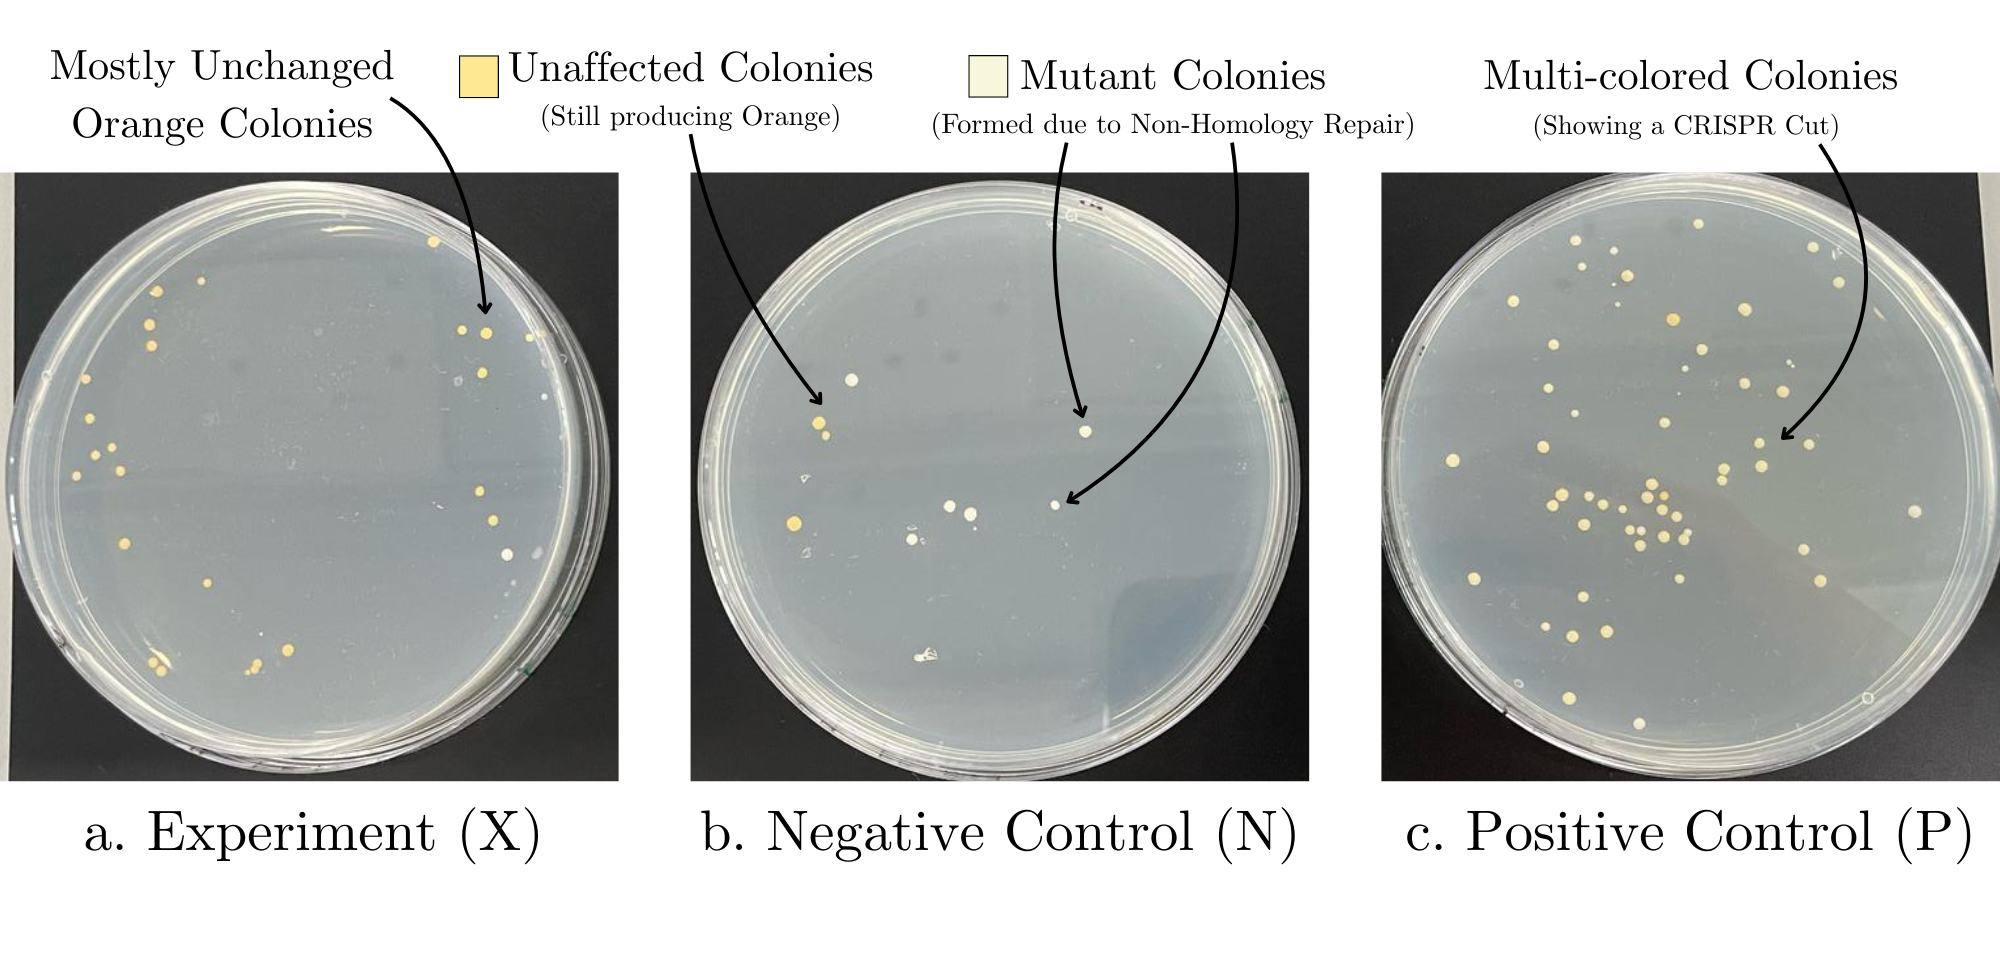
\includegraphics[width=\textwidth]{figures/exp_3_agar_plates.png}
    \caption{\centering The figures above show three plates: Experiment (X), Control (C), and Negative (N). }\label{fig:exp_3_agar_plates}
\end{figure}

\subsection{Discussion of the Results}
The Experimental plate (X) had our donor DNA and gRNA choice; negative control
(N) had no donor DNA and our CRISPR gRNA-18 construct; positive control (C) had
gRNA-9 construct with donor DNA prepared by the GTAs. The Neative Control (N)
plate shows a few orange colonies (2 to 3) where as the rest of the colonies
seem off white to light yellow in color. Difference from the original Orange
hue suggests that the CRISPR construct was successful in making the DNA edit
but due to the absence of a donor DNA, non-homologous end joining was used to
repair the cut DNA which led to random mutations (INDELS) leading to off-color
colonies. As the PAM site was not modified (again due to the absence of donor
DNA), the DNA seemed to have been repeatedly cut again and again leading to
death of many colonies. This explains the low number of colonies on the
Negative Control (N) plate.

The Positive Control (C) plate has significantly more amount of colonies as
compared to the other two plates. This plate has the gRNA-9 construct with
donor DNA prepared by the GTAs. The colonies on this plate also display a small
diversity of colors (primarily light yellow to orange). This suggests that the
CRISPR transformation (with G-9) was successful in making transforming the
CRT-I gene. The results, however, do not show a significant difference in the
B-carotene producted as compared to the saturated orange colonies from the
Negative Control (N) plate that were supposedly unaffected by the CRISPR
construct.

The Experimental (X) plate also shows very few colonies with most being
saturated orange in color (with the exception of a few light yellow and
off-white colonies). This suggests that the CRISPR transformation was
successful in making the most of DNA edits but the colonies were not able to
grow as compared to the Positive Control (C) plate. This suggests that the PAM
site was not modified as expected and the DNA went multiple rounds of cleavage
and repair leading to death of many colonies. There also doesn't seem to be any
difference in the amount of B-carotene produced as compared to the Positive
Control (C) plate.

\subsection{What would you have done with more time in the lab?}
With more time in the lab, I would have liked to do a redudant copy of the
entire experiment. In retrospect, the strategy I used to identify the colonies
to be streaked was still not properly calibrated and was a bit random. With
more time, I would probably carefully identify the colonies in the increasing
order of their color gradient to better judge the outcomes of the earlier
experiments.

\section{Yeast BioArt Picture}
\begin{figure}[h]
    \centering
    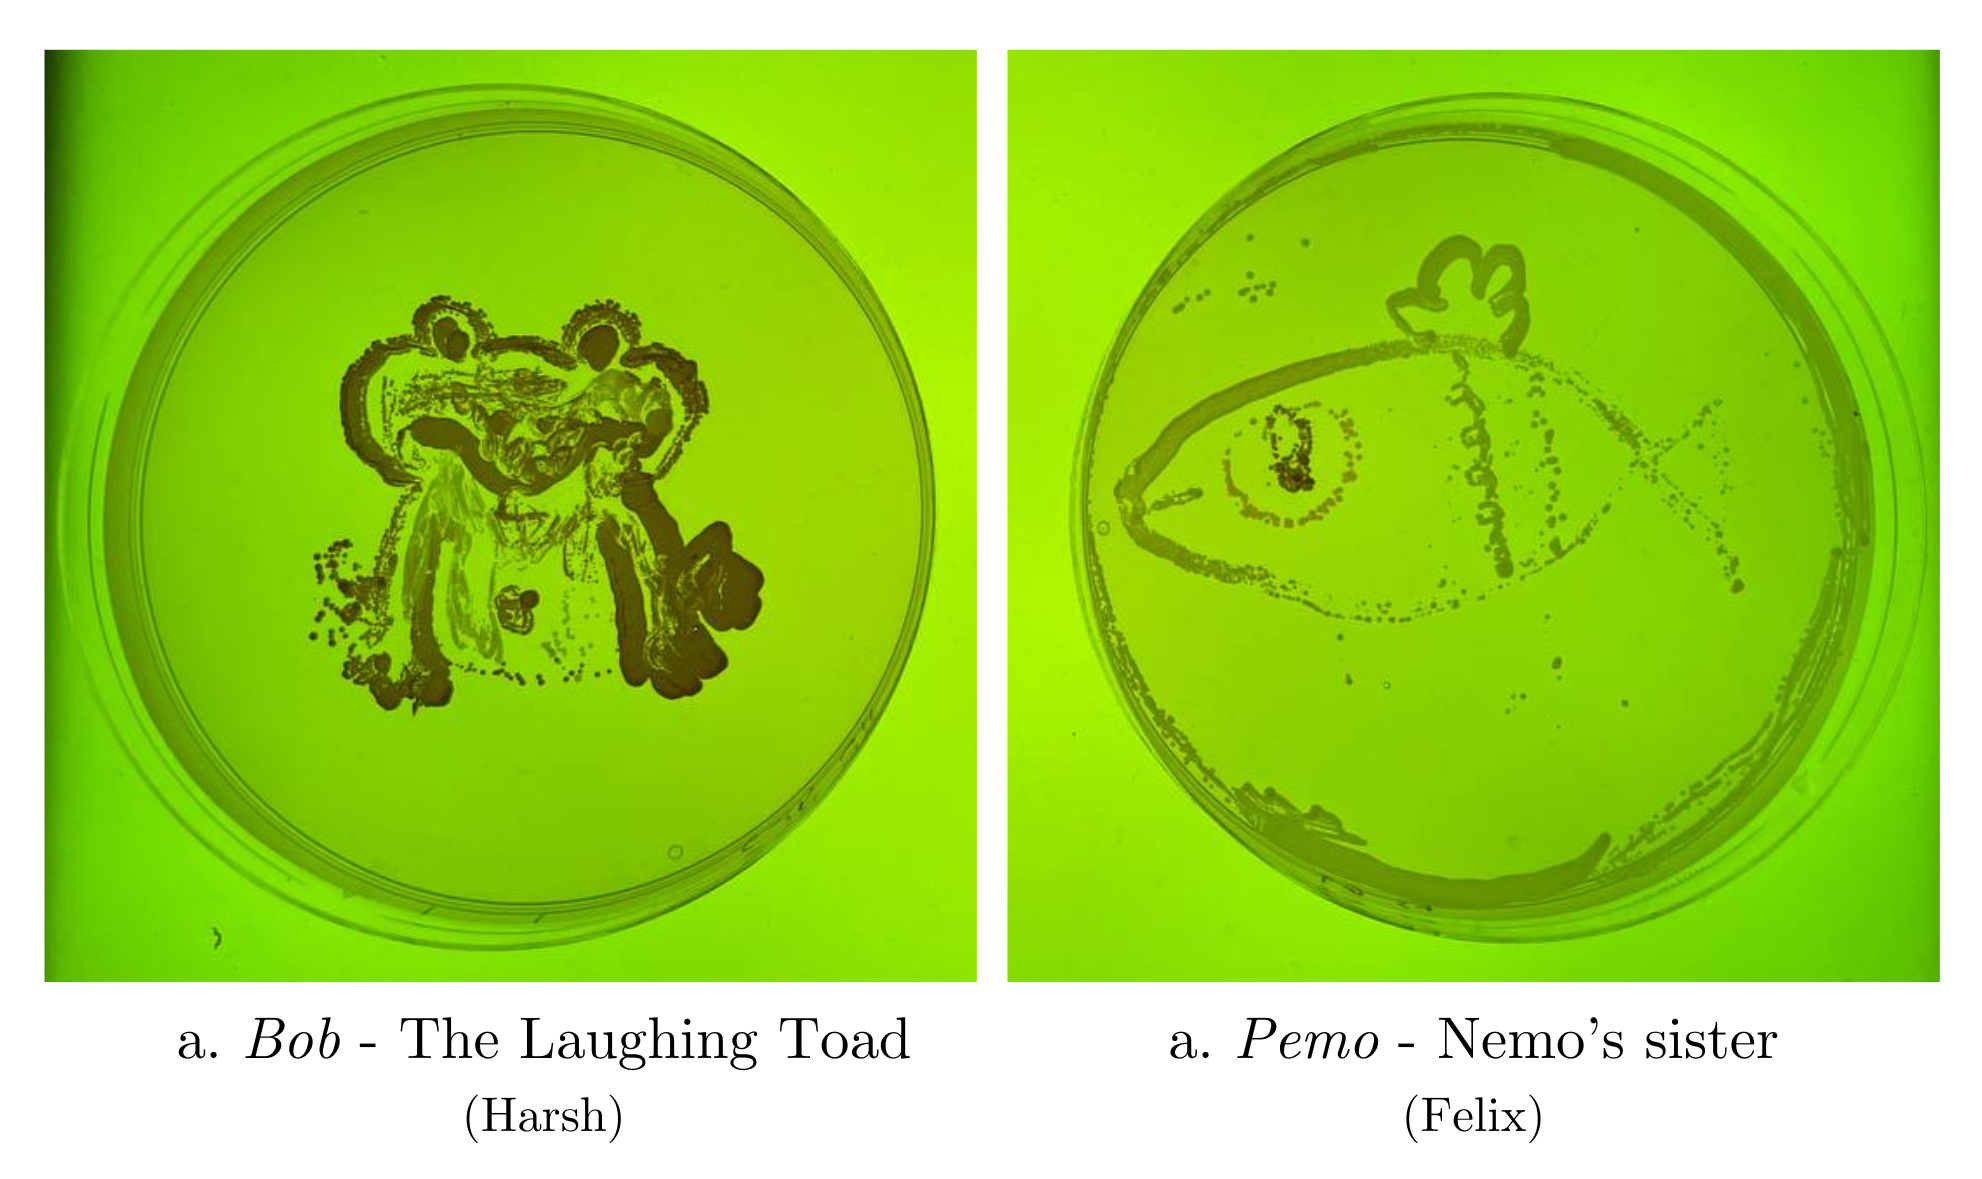
\includegraphics[width=0.8\textwidth]{figures/bioart.png}
    \caption{\centering The figures above show our attempt in Yeast Bioart.}\label{fig:bioart}
\end{figure}

I was trying to make a laughing toad (which I named Bob). Brown color was
chosen for the outline with green infill. The outcome resembles my initial
design inspiration but didn't turn out as magnificent as I hoped. My lab
partner tried to draw a fish with a `Sharingan (A visual ability from Naruto
Anime)' in its eye. While the fish's scaffold is prudent, I warned him that
drawing the eye was too ambitious.

\newpage
\section{Optimizing the Beta-Carotene Pathway in E. Coli using RBS Calculator}

\subsection{RBS Sequences for the Genes}

\begin{table}[h]
    \centering
    \begin{tabular}{|p{1.5cm}|p{14cm}|}
        \hline
        \textbf{\centering Gene} & \textbf{\centering Sequence}                                                                                                  \\
        \hline
        Crt-E                    & \texttt{\textcolor{gray}{ATACTAGAG}\textcolor{blue}{GAGGTACTAG}ATG\textcolor{gray}{ACGGTCTGCGCAAAAAAACACGTTCATCTCACTCGCGATGCT
        GCGGA}}                                                                                                                                                  \\
        \hline
        Crt-B                    & \texttt{\textcolor{gray}{CAGGCCTGGTTTGACAAAAAACTCGCTGCCGTCAGTTAATAATACTAGAG}\textcolor{blue}{CTCAAGGAGGTACT
        AG}ATG\textcolor{gray}{AATAATCCGTCGTTACTCAATCATGCGGTCGAAACGATGGCAGTTGG}}                                                                                 \\
        \hline
        Crt-I                    & \texttt{\textcolor{gray}{CCTCCCCGCCCTGCGCATCTCTGGCAGCGCCCGCTCTAATAATACTAGAG}\textcolor{blue}{CTCAAGGAGGTACT
        AG}ATG\textcolor{gray}{AAACCAACTACGGTAATTGGTGCAGGCTTCGGTGGCCTGGCACTGGC}}                                                                                 \\
        \hline
        Crt-Y                    & \texttt{\textcolor{gray}{AAAGCGACAGCAGGTTTGATGCTGGAGGATCTGATATAATAATACTAGAG}\textcolor{blue}{GAGGTACTAG}ATG\textcolor{gray}{C
        AACCGCATTATGATCTGATTCTCGTGGGGGCTGGACTCGCGAATGG}}                                                                                                         \\
        \hline
    \end{tabular}
    \caption{\centering Table shows the RBS sequences for the genes (highlighted in \textcolor{blue}{blue}) and their flanking sequences ($\approx 50$ bp each) upstream and downstream (highlighted in \textcolor{gray}{gray}). The start codon of the CDR region is highlighted in \textcolor{black}{black}.}\label{tab:rbs_gene_sequences}
\end{table}

\subsection{RBS Strength Calculation Results}

\begin{table}[h]
    \centering
    \begin{tabular}{|l|c|c|}
        \hline
        \textbf{Gene} & Translation Rate & $\Delta G_{total}$ \\
        \hline
        Crt-E         & 2672.46          & -1.72              \\
        \hline
        Crt-B         & 21787.90         & -6.38              \\
        \hline
        Crt-I         & 676.81           & 1.33               \\
        \hline
        Crt-Y         & 6069.20          & -3.54              \\
        \hline
    \end{tabular}
    \caption{\centering Table shows the predicted Translation Rate and $\Delta G_{total}$ for the genes.}\label{tab:rbs_strength}
\end{table}

\subsection{Rationale behind the gene to optimize}
The analysis of the RBS binding strengths for the beta-carotene biosynthesis
genes in table~\ref{tab:rbs_strength} shows that CRT-I, with a low translation
rate of 676.81 and a positive Delta G of 1.33 kcal/mol, is a potential
bottleneck in the pathway, limiting phytoene desaturation compared to the
higher rates of CRT-E (2672.46), CRT-B (21787.99), and CRT-Y (6069.20). To
address this, the most apt target is CRT-I, targeting a translation rate of
8000 to 10000 to enhance binding stability and align CRT-I expression with
upstream (CRT-E) and downstream (CRT-Y) flux, while avoiding the excessive
overexpression suggested by CRT-B.

\subsection{Optimized RBS Sequence for CRT-I}

\begin{table}[h]
    \centering
    \begin{tabular}{|l|c|c|c|}
        \hline
        \textbf{Gene} & \textbf{Optimized Sequence} & \textbf{Translation Rate} & \textbf{$\Delta G_{total}$} \\
        \hline
        CRT-I         & CAAGAGAAATCACATAGGGATCATTAA & 8578.85                   & -4.31                       \\
        \hline
    \end{tabular}
    \caption{\centering Table shows the original and optimized RBS sequences for CRT-I.}\label{tab:optimized_rbs}
\end{table}

\subsection{Discussion of the Results}
Optimizing the CRT-I RBS to increase its translation rate from 676.81 to
8578.85 would likely alleviate the bottleneck in the beta-carotene biosynthesis
pathway by enhancing phytoene desaturase production, ensuring better conversion
of phytoene to lycopene and supporting downstream beta-carotene synthesis. The
potential downside, however, might be that the predicted translation rate of
the new RBS sequence might be too high, potentially causing lycopene
accumulation if downstream CRT-YB cannot keep up, risking intermediate toxicity
or metabolic burden, as seen with smaller colonies. However, this is difficult
to comment out without experimental validation.

\bibliographystyle{plainnat}
\bibliography{references}

\end{document}